
%% bare_conf.tex
%% V1.3
%% 2007/01/11
%% by Michael Shell
%% See:
%% http://www.michaelshell.org/
%% for current contact information.
%%
%% This is a skeleton file demonstrating the use of IEEEtran.cls
%% (requires IEEEtran.cls version 1.7 or later) with an IEEE conference paper.
%%
%% Support sites:
%% http://www.michaelshell.org/tex/ieeetran/
%% http://www.ctan.org/tex-archive/macros/latex/contrib/IEEEtran/
%% and
%% http://www.ieee.org/

%%*************************************************************************
%% Legal Notice:
%% This code is offered as-is without any warranty either expressed or
%% implied; without even the implied warranty of MERCHANTABILITY or
%% FITNESS FOR A PARTICULAR PURPOSE! 
%% User assumes all risk.
%% In no event shall IEEE or any contributor to this code be liable for
%% any damages or losses, including, but not limited to, incidental,
%% consequential, or any other damages, resulting from the use or misuse
%% of any information contained here.
%%
%% All comments are the opinions of their respective authors and are not
%% necessarily endorsed by the IEEE.
%%
%% This work is distributed under the LaTeX Project Public License (LPPL)
%% ( http://www.latex-project.org/ ) version 1.3, and may be freely used,
%% distributed and modified. A copy of the LPPL, version 1.3, is included
%% in the base LaTeX documentation of all distributions of LaTeX released
%% 2003/12/01 or later.
%% Retain all contribution notices and credits.
%% ** Modified files should be clearly indicated as such, including  **
%% ** renaming them and changing author support contact information. **
%%
%% File list of work: IEEEtran.cls, IEEEtran_HOWTO.pdf, bare_adv.tex,
%%                    bare_conf.tex, bare_jrnl.tex, bare_jrnl_compsoc.tex
%%*************************************************************************

% *** Authors should verify (and, if needed, correct) their LaTeX system  ***
% *** with the testflow diagnostic prior to trusting their LaTeX platform ***
% *** with production work. IEEE's font choices can trigger bugs that do  ***
% *** not appear when using other class files.                            ***
% The testflow support page is at:
% http://www.michaelshell.org/tex/testflow/



% Note that the a4paper option is mainly intended so that authors in
% countries using A4 can easily print to A4 and see how their papers will
% look in print - the typesetting of the document will not typically be
% affected with changes in paper size (but the bottom and side margins will).
% Use the testflow package mentioned above to verify correct handling of
% both paper sizes by the user's LaTeX system.
%
% Also note that the "draftcls" or "draftclsnofoot", not "draft", option
% should be used if it is desired that the figures are to be displayed in
% draft mode.
%
\documentclass[journal,12pt]{IEEEtran}
% Add the compsoc option for Computer Society conferences.
%
% If IEEEtran.cls has not been installed into the LaTeX system files,
% manually specify the path to it like:
% \documentclass[conference]{../sty/IEEEtran}





% Some very useful LaTeX packages include:
% (uncomment the ones you want to load)


% *** MISC UTILITY PACKAGES ***
%
%\usepackage{ifpdf}
% Heiko Oberdiek's ifpdf.sty is very useful if you need conditional
% compilation based on whether the output is pdf or dvi.
% usage:
% \ifpdf
%   % pdf code
% \else
%   % dvi code
% \fi
% The latest version of ifpdf.sty can be obtained from:
% http://www.ctan.org/tex-archive/macros/latex/contrib/oberdiek/
% Also, note that IEEEtran.cls V1.7 and later provides a builtin
% \ifCLASSINFOpdf conditional that works the same way.
% When switching from latex to pdflatex and vice-versa, the compiler may
% have to be run twice to clear warning/error messages.


 



% *** CITATION PACKAGES ***
%
\usepackage{cite}
%\usepackage{stfloats}
% cite.sty was written by Donald Arseneau
% V1.6 and later of IEEEtran pre-defines the format of the cite.sty package
% \cite{} output to follow that of IEEE. Loading the cite package will
% result in citation numbers being automatically sorted and properly
% "compressed/ranged". e.g., [1], [9], [2], [7], [5], [6] without using
% cite.sty will become [1], [2], [5]--[7], [9] using cite.sty. cite.sty's
% \cite will automatically add leading space, if needed. Use cite.sty's
% noadjust option (cite.sty V3.8 and later) if you want to turn this off.
% cite.sty is already installed on most LaTeX systems. Be sure and use
% version 4.0 (2003-05-27) and later if using hyperref.sty. cite.sty does
% not currently provide for hyperlinked citations.
% The latest version can be obtained at:
% http://www.ctan.org/tex-archive/macros/latex/contrib/cite/
% The documentation is contained in the cite.sty file itself.






% *** GRAPHICS RELATED PACKAGES ***
%
\ifCLASSINFOpdf
  \usepackage[pdftex]{graphicx}
  % declare the path(s) where your graphic files are
  \graphicspath{{./images/}}
  % and their extensions so you won't have to specify these with
  % every instance of \includegraphics
  % \DeclareGraphicsExtensions{.pdf,.jpeg,.png}
\else
  % or other class option (dvipsone, dvipdf, if not using dvips). graphicx
  % will default to the driver specified in the system graphics.cfg if no
  % driver is specified.
  % \usepackage[dvips]{graphicx}
  % declare the path(s) where your graphic files are
  % \graphicspath{{../eps/}}
  % and their extensions so you won't have to specify these with
  % every instance of \includegraphics
  % \DeclareGraphicsExtensions{.eps}
\fi
% graphicx was written by David Carlisle and Sebastian Rahtz. It is
% required if you want graphics, photos, etc. graphicx.sty is already
% installed on most LaTeX systems. The latest version and documentation can
% be obtained at: 
% http://www.ctan.org/tex-archive/macros/latex/required/graphics/
% Another good source of documentation is "Using Imported Graphics in
% LaTeX2e" by Keith Reckdahl which can be found as epslatex.ps or
% epslatex.pdf at: http://www.ctan.org/tex-archive/info/
%
% latex, and pdflatex in dvi mode, support graphics in encapsulated
% postscript (.eps) format. pdflatex in pdf mode supports graphics
% in .pdf, .jpeg, .png and .mps (metapost) formats. Users should ensure
% that all non-photo figures use a vector format (.eps, .pdf, .mps) and
% not a bitmapped formats (.jpeg, .png). IEEE frowns on bitmapped formats
% which can result in "jaggedy"/blurry rendering of lines and letters as
% well as large increases in file sizes.
%
% You can find documentation about the pdfTeX application at:
% http://www.tug.org/applications/pdftex





% *** MATH PACKAGES ***
%
\usepackage[cmex10]{amsmath}
% A popular package from the American Mathematical Society that provides
% many useful and powerful commands for dealing with mathematics. If using
% it, be sure to load this package with the cmex10 option to ensure that
% only type 1 fonts will utilized at all point sizes. Without this option,
% it is possible that some math symbols, particularly those within
% footnotes, will be rendered in bitmap form which will result in a
% document that can not be IEEE Xplore compliant!
%
% Also, note that the amsmath package sets \interdisplaylinepenalty to 10000
% thus preventing page breaks from occurring within multiline equations. Use:
%\interdisplaylinepenalty=2500
% after loading amsmath to restore such page breaks as IEEEtran.cls normally
% does. amsmath.sty is already installed on most LaTeX systems. The latest
% version and documentation can be obtained at:
% http://www.ctan.org/tex-archive/macros/latex/required/amslatex/math/





% *** SPECIALIZED LIST PACKAGES ***
%
%\usepackage{algorithmic}
% algorithmic.sty was written by Peter Williams and Rogerio Brito.
% This package provides an algorithmic environment fo describing algorithms.
% You can use the algorithmic environment in-text or within a figure
% environment to provide for a floating algorithm. Do NOT use the algorithm
% floating environment provided by algorithm.sty (by the same authors) or
% algorithm2e.sty (by Christophe Fiorio) as IEEE does not use dedicated
% algorithm float types and packages that provide these will not provide
% correct IEEE style captions. The latest version and documentation of
% algorithmic.sty can be obtained at:
% http://www.ctan.org/tex-archive/macros/latex/contrib/algorithms/
% There is also a support site at:
% http://algorithms.berlios.de/index.html
% Also of interest may be the (relatively newer and more customizable)
% algorithmicx.sty package by Szasz Janos:
% http://www.ctan.org/tex-archive/macros/latex/contrib/algorithmicx/




% *** ALIGNMENT PACKAGES ***
%
%\usepackage{array}
% Frank Mittelbach's and David Carlisle's array.sty patches and improves
% the standard LaTeX2e array and tabular environments to provide better
% appearance and additional user controls. As the default LaTeX2e table
% generation code is lacking to the point of almost being broken with
% respect to the quality of the end results, all users are strongly
% advised to use an enhanced (at the very least that provided by array.sty)
% set of table tools. array.sty is already installed on most systems. The
% latest version and documentation can be obtained at:
% http://www.ctan.org/tex-archive/macros/latex/required/tools/


%\usepackage{mdwmath}
%\usepackage{mdwtab}
% Also highly recommended is Mark Wooding's extremely powerful MDW tools,
% especially mdwmath.sty and mdwtab.sty which are used to format equations
% and tables, respectively. The MDWtools set is already installed on most
% LaTeX systems. The lastest version and documentation is available at:
% http://www.ctan.org/tex-archive/macros/latex/contrib/mdwtools/


% IEEEtran contains the IEEEeqnarray family of commands that can be used to
% generate multiline equations as well as matrices, tables, etc., of high
% quality.


%\usepackage{eqparbox}
% Also of notable interest is Scott Pakin's eqparbox package for creating
% (automatically sized) equal width boxes - aka "natural width parboxes".
% Available at:
% http://www.ctan.org/tex-archive/macros/latex/contrib/eqparbox/





% *** SUBFIGURE PACKAGES ***
\usepackage[tight,footnotesize]{subfigure}
% subfigure.sty was written by Steven Douglas Cochran. This package makes it
% easy to put subfigures in your figures. e.g., "Figure 1a and 1b". For IEEE
% work, it is a good idea to load it with the tight package option to reduce
% the amount of white space around the subfigures. subfigure.sty is already
% installed on most LaTeX systems. The latest version and documentation can
% be obtained at:
% http://www.ctan.org/tex-archive/obsolete/macros/latex/contrib/subfigure/
% subfigure.sty has been superceeded by subfig.sty.



%\usepackage[caption=false]{caption}
%\usepackage[font=footnotesize]{subfig}
% subfig.sty, also written by Steven Douglas Cochran, is the modern
% replacement for subfigure.sty. However, subfig.sty requires and
% automatically loads Axel Sommerfeldt's caption.sty which will override
% IEEEtran.cls handling of captions and this will result in nonIEEE style
% figure/table captions. To prevent this problem, be sure and preload
% caption.sty with its "caption=false" package option. This is will preserve
% IEEEtran.cls handing of captions. Version 1.3 (2005/06/28) and later 
% (recommended due to many improvements over 1.2) of subfig.sty supports
% the caption=false option directly:
%\usepackage[caption=false,font=footnotesize]{subfig}
%
% The latest version and documentation can be obtained at:
% http://www.ctan.org/tex-archive/macros/latex/contrib/subfig/
% The latest version and documentation of caption.sty can be obtained at:
% http://www.ctan.org/tex-archive/macros/latex/contrib/caption/




% *** FLOAT PACKAGES ***
%
%\usepackage{fixltx2e}
% fixltx2e, the successor to the earlier fix2col.sty, was written by
% Frank Mittelbach and David Carlisle. This package corrects a few problems
% in the LaTeX2e kernel, the most notable of which is that in current
% LaTeX2e releases, the ordering of single and double column floats is not
% guaranteed to be preserved. Thus, an unpatched LaTeX2e can allow a
% single column figure to be placed prior to an earlier double column
% figure. The latest version and documentation can be found at:
% http://www.ctan.org/tex-archive/macros/latex/base/



%\usepackage{stfloats}
% stfloats.sty was written by Sigitas Tolusis. This package gives LaTeX2e
% the ability to do double column floats at the bottom of the page as well
% as the top. (e.g., "\begin{figure*}[!b]" is not normally possible in
% LaTeX2e). It also provides a command:
%\fnbelowfloat
% to enable the placement of footnotes below bottom floats (the standard
% LaTeX2e kernel puts them above bottom floats). This is an invasive package
% which rewrites many portions of the LaTeX2e float routines. It may not work
% with other packages that modify the LaTeX2e float routines. The latest
% version and documentation can be obtained at:
% http://www.ctan.org/tex-archive/macros/latex/contrib/sttools/
% Documentation is contained in the stfloats.sty comments as well as in the
% presfull.pdf file. Do not use the stfloats baselinefloat ability as IEEE
% does not allow \baselineskip to stretch. Authors submitting work to the
% IEEE should note that IEEE rarely uses double column equations and
% that authors should try to avoid such use. Do not be tempted to use the
% cuted.sty or midfloat.sty packages (also by Sigitas Tolusis) as IEEE does
% not format its papers in such ways.





% *** PDF, URL AND HYPERLINK PACKAGES ***
%
%\usepackage{url}
% url.sty was written by Donald Arseneau. It provides better support for
% handling and breaking URLs. url.sty is already installed on most LaTeX
% systems. The latest version can be obtained at:
% http://www.ctan.org/tex-archive/macros/latex/contrib/misc/
% Read the url.sty source comments for usage information. Basically,
% \url{my_url_here}.





% *** Do not adjust lengths that control margins, column widths, etc. ***
% *** Do not use packages that alter fonts (such as pslatex).         ***
% There should be no need to do such things with IEEEtran.cls V1.6 and later.
% (Unless specifically asked to do so by the journal or conference you plan
% to submit to, of course. )


% correct bad hyphenation here
\hyphenation{op-tical net-works semi-conduc-tor}
\usepackage{listings}
\usepackage{amsfonts}
\graphicspath{{./img/}}
\begin{document}
%
% paper title
% can use linebreaks \\ within to get better formatting as desired



% author names and affiliations
% use a multiple column layout for up to three different
% affiliations
\title{\vspace{-0.05\textheight}Human Computer Interaction 2011\\\large{Assignment 1: Image Labelling Application}}

\author{
\IEEEauthorblockN{Behzad Tabibian and William Ogilvie}\\
\IEEEauthorblockA{School of Informatics\\University of Edinburgh\\}
}


% conference papers do not typically use \thanks and this command
% is locked out in conference mode. If really needed, such as for
% the acknowledgment of grants, issue a \IEEEoverridecommandlockouts
% after \documentclass

% for over three affiliations, or if they all won't fit within the width
% of the page, use this alternative format:
% 
%\author{\IEEEauthorblockN{Michael Shell\IEEEauthorrefmark{1},
%Homer Simpson\IEEEauthorrefmark{2},
%James Kirk\IEEEauthorrefmark{3}, 
%Montgomery Scott\IEEEauthorrefmark{3} and
%Eldon Tyrell\IEEEauthorrefmark{4}}
%\IEEEauthorblockA{\IEEEauthorrefmark{1}School of Electrical and Computer Engineering\\
%Georgia Institute of Technology,
%Atlanta, Georgia 30332--0250\\ Email: see http://www.michaelshell.org/contact.html}
%\IEEEauthorblockA{\IEEEauthorrefmark{2}Twentieth Century Fox, Springfield, USA\\
%Email: homer@thesimpsons.com}
%\IEEEauthorblockA{\IEEEauthorrefmark{3}Starfleet Academy, San Francisco, California 96678-2391\\
%Telephone: (800) 555--1212, Fax: (888) 555--1212}
%\IEEEauthorblockA{\IEEEauthorrefmark{4}Tyrell Inc., 123 Replicant Street, Los Angeles, California 90210--4321}}




% use for special paper notices
%\IEEEspecialpapernotice{(Invited Paper)}




% make the title area
\maketitle


%\begin{abstract}
%\boldmath
%The abstract goes here.
%\end{abstract}
% IEEEtran.cls defaults to using nonbold math in the Abstract.
% This preserves the distinction between vectors and scalars. However,
% if the conference you are submitting to favors bold math in the abstract,
% then you can use LaTeX's standard command \boldmath at the very start
% of the abstract to achieve this. Many IEEE journals/conferences frown on
% math in the abstract anyway.

% no keywords




% For peer review papers, you can put extra information on the cover
% page as needed:
% \ifCLASSOPTIONpeerreview
% \begin{center} \bfseries EDICS Category: 3-BBND \end{center}
% \fi
%
% For peerreview papers, this IEEEtran command inserts a page break and
% creates the second title. It will be ignored for other modes.
\IEEEpeerreviewmaketitle
	


\section{Introduction}
Here goes the introduction
\section{Experimental Procedure}

The experiment was initially going to be run on a Linux Laptop, since that was the most convenient to hand, but had to moved to a Windows Desktop machine when a fairly sizable bug was discovered.  It turns out that the icons in the application window do not display correctly when viewed on a lower resolution screen (1366 x 768 in this case) - see figure 1.  This is clearly bad interface design in that the creators of the product did not envisage it to be used on a screen resolution that was smaller than the one they evidently implemented it on.  This flaw makes the system potentially unusable to a number of users, and so if this were a real scenario this bug would need to be corrected before this program were released to the general public.

\begin{figure}[t]
\centering
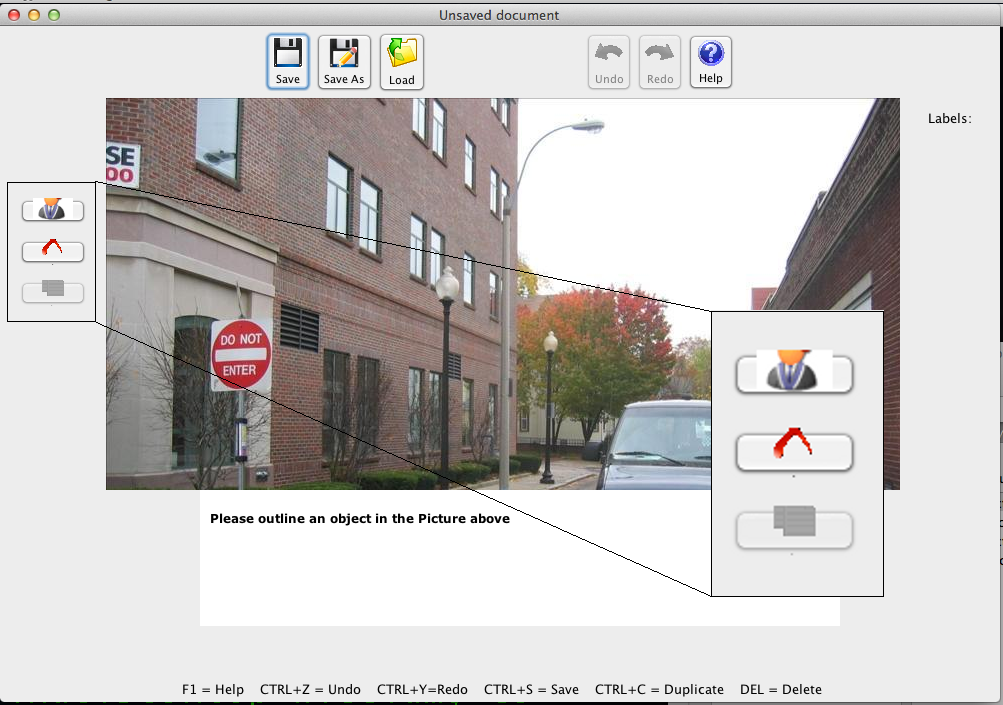
\includegraphics[width=6cm]{sshot2.png}
\caption{A screen-shot of the main window of the application, notice that the zoomed in section has buttons which are squashed causing them to appear to have no label or legible icon}
\label{fig:fullView}
\end{figure}

Having found a monitor that had a large enough resolution display the participant was briefed on what the product was intended to be used for and then asked to give their initial impressions on the interface design.  They were then instructed to carry out several tasks to exercise the full functionality of the program whilst being timed, with the number of mouse clicks required per task also being recorded.  After the successful completion of each operation the thoughts of the participant were taken and they were asked to give a score out of five with regards to how easy they found it to accomplish: one being easy, five being hard.  The tasks were to load an image file, add an annotation, create a second annotation, select an annotation, delete an annotation, edit an annotation, duplicate an annotation, and finally save the annotated image.  This process was repeated three times for an image labelled A, an image labelled B, and finally back to image A.  The purpose of this technique was to observe how the user gained familiarity with the product over time and to ensure they could return to a previously edited file after leaving it.

In the following sections we will discuss what the participant’s thoughts were at each stage of the test and then analyse how those relate to the principles of human-computer interactions.

\section{Results}

At the outset of the test, after an explanation of what the product was intended to allow a person to achieve, the interface was shown to the participant and they were asked to give their initial impressions.  One of the first things they noted about the application was the lack of what they felt was a “standard” layout.  More specifically, they commented on how there was no main menu present at the top of the window but instead large labelled action buttons arranged around the primary canvas area.  However, they also said that they thought it looked pretty straight forward to use by appearance alone.

The first test was to load an image file that had been placed on the user’s desktop.  This took 56 seconds to complete but only five clicks of the mouse.  The operation took a relatively long time because some considerable searching was required by the user to find the relevant button.  This confusion was attributed by them to the lack of a File menu with an Open item which they feel is fairly standard in most applications they use.  The participant scored it a 3 out of 5 for usability and said that it was easy enough to do, they just couldn’t find the right user interface control to start the operation.

The second and third tests were to add an annotation followed by a second annotation.  On both occasions the participant successfully created them in around five seconds with slight variances in the number of clicks required relating directly to the size of the polygon they drew.  They found this extremely simple and gave this feature a usability rating of one - meaning easy.

The fourth task they were set was to select a previously created annotation and this took 43 seconds to complete with five clicks required.  Initially there was some confusion during this test because the user tried to click on the edge of the polygon to select it.  When this didn’t work, and they ended up creating another polygon by mistake, they hunted around looking at the interface more closely.  Eventually they discovered the labels of the annotations on the far right of the window and completed the selection.  The participant stated that they would have preferred if the list of annotations were placed in a more prominent position and gave this feature a 3 out of 5.

The fifth task was to delete an annotation that they had made.  This took 6 seconds to complete with only one click.  The user said that they were happy that this was an easy operation giving it a score of one.

The sixth test was to edit an annotation.  The user was prompted to increase the size of their polygon and then to change its name.  These actions took 8 and 15 seconds respectively with a click required for each.  The participant stated that again this was an easy operation to complete but that they wished the list of annotations were nearer the canvas area.  They gave this a score of 2

Duplicating an annotation was the seventh task and was completed in two clicks over a period of four seconds.  This was considered easy by the test’s participant and they gave this a score of 1.

The final task asked of the user was to save the annotated image to a file.  This took seven seconds, two clicks, and they stated it was extremely easy, again giving this a score of one.  This experiment was then repeated for a second image and then again for the first image.  All measurements recorded for these subsequent operations can be seen in the appendix.

\section{Menu and Shortcuts}

Overall the participant in our tests found the program to be easy to use after a few tries, but there were a few stumbling blocks they encountered whilst using the program.  Namely these related to the placement of user interface components and the implementation of the canvas.

It took the user 56 seconds in total to load an image file, and most of that time was spent hunting the interface for the open command.  The creators of the application labelled their button load, which is arguably a less common term than open, but the main problem that the user encountered was that the vast majority of desktop applications they have used have a main menu with a file sub-menu and an open menu item - this program does not.  Also, because the action buttons seem fairly arbitrarily placed around the canvas, this will necessarily add to the confusion of first-time users.

The other task that the user found particularly difficult was the selecting of an annotation.  This took them 45 seconds to complete, and in terms of poor interface design there were two main issues.  The first thing that the user tried to do was select the edge of the polygon to highlight it.  This is a fairly natural action since it is usually the case that a UI object can be selected by clicking on it; however, in this case the canvas interpreted the click incorrectly as the users wish to create another polygon.  This is poor interface design since the designers of the program should have imagined that the user would try to select an annotation in this way and either implement it or communicate to the user that the edges of the polygon are not click-able: perhaps by using a broken line as opposed to a continuous one.  After the user recovered from their error they realised that the selection of an annotation must be accomplished somewhere else on the window and this illustrates the second issue with this feature.  It took some time for the participant of the test to realise there was a list of their annotations to the far right of the window.  User interface components are typically placed to the top and the left of the screen so by placing a piece of information on the far right it is less likely that a persons eye will travel that way as often.  This is fairly well known in interface design, and so the creators of this product should have given more thought to the placement and implementation of this feature.

\section{Conclusion}

In conclusion, the participant in our tests seemed happy with the program after learning how to use it.  However, looking at the interface implementation from a more professional point of view it is clear that some mistakes have been made.  For one thing, there should not be a 50 second plus learning curve on opening an image file.  This is one of the simplest operations a desktop application can make, and this confusion was entirely avoidable had the designers taken the time to implement the standard main menu, File sub-menu pattern found in so many applications.

Having ignored that convention, the programmers placed a vital user interface element at the far right of the window. It is well known in design, and has be born out by research carried out into eye movement tracking, that a person concentrates their gaze to the top and left of an application.  By placing the list of annotations on the far right they should have considered that it may be more difficult for a user to spot, and consequently re-thought that placement.  

Finally, it is typical in every day computer use that clicking on a UI component will either highlight or select it.  By separating the place where you select an annotation from the place where it is drawn you are disregarding this paradigm, and ultimately this may lead to the confusion of users.

Design deficiencies are clearly demonstrated in Figure \ref{fig:ave_rate} when the time to complete a task for the first time is plotted against user rating of how easy the task was.

\begin{figure}[t]
\centering
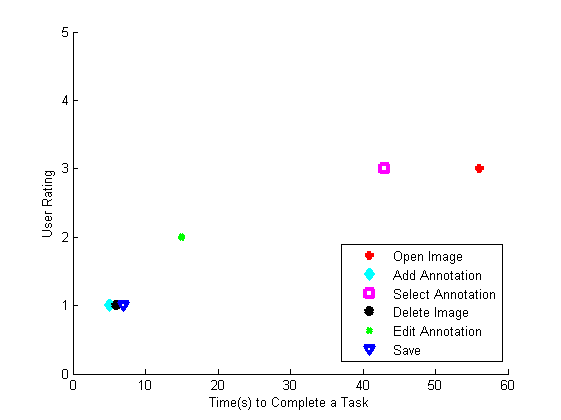
\includegraphics[width=8cm]{average_rating.png}
\caption{time takes for completing a task for the first time plotted against user rating of how easy it was to accomplish the task, lower number indicates task was easier. }
\label{fig:ave_rate}
\end{figure}

Since the application has fairly simple use cases it does get away with having a bit of a quirky layout, at least as far as our test subject was concerned.  However, in terms of following HCI principles, this application breaches a few too many and so we feel it would be better to redo the design in a more conventional manner so that users may be less confused while using it.

\renewcommand{\appendixname}{Appendix A}
\newpage
\appendix
\section{Mathematical Derivation of Bayesian Inference Engine}
Every possible action of the user can be shown as a vector: $X_{act}=(open, save, edit, add)^T$ in which  $act \in {open, save, edit, add}$. Every action can be modelled as a \textit{Multinomial Distribution}:

\[
Mult(m_1,m_2,...,m_K|\mu,N)={N \choose m_1 m_2 ... m_K}\prod_{k=1}^K \mu_{k}^{x_k}
\]

where $\mu=(\mu_1,\mu_2,...,\mu_K)^T$. Finding the maximum likelihood solution for parameter $\mu$ will give us:

\[
\mu_k^{ML}={m_k \over N} 
\]

We use this result to approximate the best probability for the next action. It is natural to think about this result as averaging over the observations.
To take one step further and introduce priors to the distribution we use \textit{Dirichlet distribution} which is the conjugate prior of the multinomial distribution.
\[
Dir(\mu|\alpha)={\Gamma(\alpha_0) \over \Gamma(\alpha_1)...\Gamma(\alpha_K)}\prod_{k=1}^K \mu_{k}^{\alpha_k -1}
\]
Conjugate priors have certain characteristics which makes it easy to compute the posterior of the distribution that is constructed by multiplying the likelihood function by the prior.  
\[
p(D|\mu)=\prod_{k=1}^K {\mu_{k}^{m_k}}\]

\[p(\mu| D,\alpha) \propto p(D|\mu)  p(\mu|\alpha)\]

\[p(\mu|D, \alpha)={\Gamma(\alpha_0+N) \over {\Gamma(\alpha_1+m_1)...\Gamma(\alpha_K+m_K)}}\prod_{k=1}^K \mu_{k}^{\alpha_k+m_k-1}\]

Marginalizing over $\mu$ we get 

\[p(x=add|D)=\int_0^1 p(x=add|\mu)p(\mu|D) \mathrm{d}\mu\]
\[p(x=add|D)=\int_0^1 \mu p(\mu|D)\mathrm{d}\mu = \mathbb{E}[\mu|D]\]

The value of the last line is equal to

\[\mathbb{E}[\mu|D]={m_k+\alpha_k \over {N+\alpha_0}} \]

The result, just like earlier, can be interpreted as considering priors as imaginary observations.

After calculating the $\mu$ of every action the suggestion is produced by using the Inverse Transform method and a uniform distribution.

In conclusion, the resulting model even though simple is tractable and produces expected results which are fairly robust.

For further information the reader is referred to \cite{Bishop2007}. 

\bibliographystyle{IEEEtran}
\bibliography{bibliography}


% An example of a floating figure using the graphicx package.
% Note that \label must occur AFTER (or within) \caption.
% For figures, \caption should occur after the \includegraphics.
% Note that IEEEtran v1.7 and later has special internal code that
% is designed to preserve the operation of \label within \caption
% even when the captionsoff option is in effect. However, because
% of issues like this, it may be the safest practice to put all your
% \label just after \caption rather than within \caption{}.
%
% Reminder: the "draftcls" or "draftclsnofoot", not "draft", class
% option should be used if it is desired that the figures are to be
% displayed while in draft mode.
%
%\begin{figure}[!t]
%\centering
%\includegraphics[width=2.5in]{myfigure}
% where an .eps filename suffix will be assumed under latex, 
% and a .pdf suffix will be assumed for pdflatex; or what has been declared
% via \DeclareGraphicsExtensions.
%\caption{Simulation Results}
%\label{fig_sim}
%\end{figure}

% Note that IEEE typically puts floats only at the top, even when this
% results in a large percentage of a column being occupied by floats.


% An example of a double column floating figure using two subfigures.
% (The subfig.sty package must be loaded for this to work.)
% The subfigure \label commands are set within each subfloat command, the
% \label for the overall figure must come after \caption.
% \hfil must be used as a separator to get equal spacing.
% The subfigure.sty package works much the same way, except \subfigure is
% used instead of \subfloat.
%
%\begin{figure*}[!t]
%\centerline{\subfloat[Case I]\includegraphics[width=2.5in]{subfigcase1}%
%\label{fig_first_case}}
%\hfil
%\subfloat[Case II]{\includegraphics[width=2.5in]{subfigcase2}%
%\label{fig_second_case}}}
%\caption{Simulation results}
%\label{fig_sim}
%\end{figure*}
%
% Note that often IEEE papers with subfigures do not employ subfigure
% captions (using the optional argument to \subfloat), but instead will
% reference/describe all of them (a), (b), etc., within the main caption.


% An example of a floating table. Note that, for IEEE style tables, the 
% \caption command should come BEFORE the table. Table text will default to
% \footnotesize as IEEE normally uses this smaller font for tables.
% The \label must come after \caption as always.
%
%\begin{table}[!t]
%% increase table row spacing, adjust to taste
%\renewcommand{\arraystretch}{1.3}
% if using array.sty, it might be a good idea to tweak the value of
% \extrarowheight as needed to properly center the text within the cells
%\caption{An Example of a Table}
%\label{table_example}
%\centering
%% Some packages, such as MDW tools, offer better commands for making tables
%% than the plain LaTeX2e tabular which is used here.
%\begin{tabular}{|c||c|}
%\hline
%One & Two\\
%\hline
%Three & Four\\
%\hline
%\end{tabular}
%\end{table}


% Note that IEEE does not put floats in the very first column - or typically
% anywhere on the first page for that matter. Also, in-text middle ("here")
% positioning is not used. Most IEEE journals/conferences use top floats
% exclusively. Note that, LaTeX2e, unlike IEEE journals/conferences, places
% footnotes above bottom floats. This can be corrected via the \fnbelowfloat
% command of the stfloats package.

% conference papers do not normally have an appendix


% use section* for acknowledgement




% trigger a \newpage just before the given reference
% number - used to balance the columns on the last page
% adjust value as needed - may need to be readjusted if
% the document is modified later
%\IEEEtriggeratref{8}
% The "triggered" command can be changed if desired:
%\IEEEtriggercmd{\enlargethispage{-5in}}

% references section

% can use a bibliography generated by BibTeX as a .bbl file
% BibTeX documentation can be easily obtained at:
% http://www.ctan.org/tex-archive/biblio/bibtex/contrib/doc/
% The IEEEtran BibTeX style support page is at:
% http://www.michaelshell.org/tex/ieeetran/bibtex/
%\bibliographystyle{IEEEtran}
% argument is your BibTeX string definitions and bibliography database(s)
%\bibliography{IEEEabrv,../bib/paper}
%
% <OR> manually copy in the resultant .bbl file
% set second argument of \begin to the number of references
% (used to reserve space for the reference number labels box)
%\begin{thebibliography}{1}

%\bibliographystyle{IEEEtran}
%\bibliography{bibliography}

%\end{thebibliography}




% that's all folks
\end{document}


